\documentclass[a4paper]{article}
\usepackage[brazil]{babel}
\usepackage[utf8]{inputenc}
\usepackage[backend=bibtex]{biblatex}
\usepackage{listings}
\usepackage{color}
\usepackage{graphicx}
\usepackage{float}
\usepackage[textheight=25cm, textwidth=15cm]{geometry}

\renewcommand{\lstlistingname}{Algoritmo}
\lstset{
	language=C++,
	basicstyle=\ttfamily,
	numbers=left,
	numberstyle=\small,
	frame=tb,
	tabsize=2,
	columns=fixed,
	showstringspaces=false,
	showtabs=false,
	keepspaces,
	commentstyle=\color{red},
	keywordstyle=\color{blue}
}


\bibliography{references.bib}

%opening
\title{Programação concorrente - Cozinha de Fast Food}
\author{Victor Costa}

\begin{document}

\maketitle

\section{Introdução}
\label{sec:introduction}

Este artigo tem por objetivo simular a concorrência correta de uma cozinha de um restaurante de \textit{fast-food}. Em um restaurante de \textit{fast-food} típico as tarefas que existem giram em torno de anotar e entregar pedidos, preparar comida, limpar o ambiente e reestocar ingredientes. Para o propósito educacional desse problema o foco será na entrega de pedidos e preparação de hambúrgueres e porções de batatas fritas. Para a recepção de pedidos assume-se que os clientes conseguem pedir sozinhos. As outras tarefas são consideradas magicamente feitas.

Para a resolução desse problema será utilizada a biblioteca \textit{pthread} e a linguagem de programação C++ versão de 2011 (\texttt{-std=c++11}). Essa biblioteca fornece funções para gerenciamento de \textit{threads} e a sincronização delas. Para resolver este problema optou-se por usar \textit{locks} e variáveis de condição.

\section{Formalização do problema}
\label{sec:definingTheProblem}

O objetivo é simular um restaurante. Este restaurante é de \textit{fast-food} e nele se vende hambúrgueres e porções de batata frita apenas. Os clientes fazem pedidos através de um totem que disponibiliza os pedidos para os funcionários do restaurante automaticamente. Após receber um pedido, funcionários deverão operar as máquinas e estações para atender ao pedido do primeiro cliente da fila. As máquinas e estações que existem são:

\begin{itemize}
	\item Fritadeira: frita batatas sozinha. Para funcionar precisa de um preparo feito por algum funcionário. Ela automaticamente frita e disponibiliza uma quantidade de batatas fritas sem sal.

	\item Estação de salgagem de fritas: após fritar, as batatas precisam de sal e de serem colocadas em caixas. Esta estação necessita de toda a atenção do funcionário Uma fritada das fritadeiras permite que se façam mais de uma porção de batatas fritas.

	\item Chapa: o funcionário frita as carnes dos hambúrgueres aqui. Este equipamento exige toda a atenção do chapeiro, porém no fim frita várias carnes de uma vez.

	\item Estação de montagem de hambúrgueres: após fritar as carnes, precisa-se montar o hambúrguer com todos os outros ingredientes. Nesta estação o funcionário mantém toda sua concentração e no fim do processo gera apenas um hambúrguer pronto.

	\item Balcão de entrega: aqui o funcionário gasta um tempo montando o pedido do primeiro na fila e entrega a ele. Exige toda a atenção do funcionário.
\end{itemize}


Os valores dos parâmetros de tempo, quantidade de comida gerada por tarefa e quantidade de funcionários por estação não são relevantes para a resolução do problema, então foram todos deixados como constantes configuráveis no programa. Todas as estações têm limite de funcionários operando que deve ser observado na resolução do problema. Todos os funcionários só conseguem realizar uma tarefa por vez.

\section{Descrição do algoritmo da solução do problema}
\label{sec:algorithmDescription}

\subsection{Principais desafios}
\label{sec:biggestChallenges}

Este problema está cheio de condições de corrida, mas elas essencialmente consistem de 2 tipos: limitar quantidade de trabalhadores e garantir a validade das quantidades de comida produzidas. O primeiro tipo aparece quando existem múltiplos funcionários tentando acessar a mesma máquina e é resolvido com uma variável de controle que exige acesso exclusivo. O segundo tipo ocorre no momento em que uma estação produz um recurso que outra quer utilizar e para resolver a variável que cuida da quantidade do recurso só pode ser acessada exclusivamente.

Existem também problemas de possíveis \textit{deadlocks} no momento da aquisição de múltiplos recursos. Para resolver isso, todas as funções foram conferidas na ordem que eram chamadas para remover ciclos de requisitos e em momentos de requisição de múltiplos \textit{locks}, eles sempre foram adquiridos em uma ordem única para o programa.

Além desses desafios, deve-se deixar as \textit{threads} dormindo em momentos que não têm tarefas para realizar. Ao retirar esperas ocupadas evita-se \textit{starvation} de linhas de execução e otimiza-se o uso do processador. Para isso fez-se uso extensivo de variáveis de condição.

\subsection{Resolvendo condições de corrida}

\subsubsection{Retirada segura de recursos}
\label{sec:safeResourceRemoval}

A primeira condição de corrida se refere a retirada de um recurso para uso em outra tarefa. Nela asseguramos que o valor do recurso é consistente, evitando itens fantasma e sumiço de itens. Para não ter que compartilhar o \textit{lock} com outros módulos, optou-se for fazer uma função que testa e retira. O algoritmo \ref{lst:safeResourceRemoval} implementa a solução desse problema.

\begin{lstlisting}[caption=Retirada segura de recursos da estação de montagem de hambúrgueres.\label{lst:safeResourceRemoval}]
bool AssemblyStation::getBurgers(int n)
{
	bool canDo = false;
	pthread_mutex_lock(&mutex);
	if (burgers >= n)
	{
		burgers -= n;
		statusDisplayer->updateAssemblyStationBurgers(burgers);
		canDo = true;
	}
	pthread_mutex_unlock(&mutex);
	
	if (!canDo)
		return false;
	
	return true;
}
\end{lstlisting}

Nas linhas 5 a 10 do algoritmo \ref{lst:safeResourceRemoval} está localizada a região crítica, onde se testa a possibilidade de remoção da quantidade recebida. O acesso exclusivo é garantido pelas linhas 4 e 11, por conta dos \textit{locks} que garantem que só uma linha de execução conseguem obter a trava. No caso de possível a retirada, ela ocorre dentro dessa mesma região. De forma a aumentar a concorrência, faz-se uso de uma variável local booleana chamada \texttt{canDo} que guarda se foi possível ou não retirar. Fora da região crítica, das linhas 13 a 16 é informado à quem chamou a função se foi possível ou não extrair o valor.

A linha 8 do algoritmo \ref{lst:safeResourceRemoval} é uma chamada a um método de uma classe responsável por mostrar o estado do restaurante de forma organizada após cada alteração. Este módulo é completamente destacável do programa e não é relevante para a resolução do problema.

\subsubsection{Limitação de funcionários e adição segura de recursos}
\label{sec:limitWorkersAndSafeAdd}

Para limitar os funcionários, faz-se um algoritmo muito parecido. A maior mudança é a condição de uso e os efeitos colaterais. A condição nas linhas 5 e 6 do algoritmo \ref{lst:limitWorkersAndSafeAdd}	limita a quantidade de trabalhadores pela variável de controle \texttt{workers} e usa a função \texttt{Griddle::getBurgerMeats}, que funciona de forma similar ao algoritmo \ref{lst:safeResourceRemoval}, para testar se tem recursos para realizar a tarefa. No caso em que ambas as condições sejam verdadeiras, ajusta-se o valor de \texttt{workers} para garantir que não sejam excedidos o número de trabalhadores nessa estação e também ajusta-se a quantidade de recursos retirada. O ajuste da quantidade retirada ocorre dentro da função \texttt{Griddle::getBurgerMeats} para não ter a necessidade de lidar com \textit{locks} de outro módulo.

Existem estações de trabalho que não precisam verificar a existência de recursos, como a fritadeira e a grelha, e nesse caso apenas retira-se da condição a função que pede por recursos.

No momento que o funcionário terminar sua tarefa (após o \texttt{sleep} da linha 16), adquire-se o \textit{lock} referente aos trabalhadores e recursos gerados da própria estação (linha 17). Tendo esta trava, o algoritmo atualiza a variável de controle \texttt{workers} para indicar que o funcionário deixou a estação de trabalho. Ao mesmo tempo é incrementada a variável dos recursos produzidos pela estação (linha 19), adicionando os recursos de forma segura.

Ao fim de toda tarefa os trabalhadores são acordados, pois uma estação ficou livre para funcionários realizarem tarefas nela. Isso será mais aprofundado na seção \ref{sec:avoidBusyWaits}.

\begin{lstlisting}[caption=Limitação de funcionários e adição segura de recursos na estação de montagem de hambúrgueres.\label{lst:limitWorkersAndSafeAdd}]
bool AssemblyStation::makeBurgers()
{
	bool canDo = false;
	pthread_mutex_lock(&mutex);
	if (workers < maxWorkers 
		&& Griddle::getBurgerMeats(burgersPerBatch))
	{
		statusDisplayer->updateAssemblyStationWorkers(++workers);
		canDo = true;
	}
	pthread_mutex_unlock(&mutex);
	
	if (!canDo)
		return false;
	
	sleep(assemblingTime);
	pthread_mutex_lock(&mutex);
	statusDisplayer->updateAssemblyStationWorkers(--workers);
	burgers += burgersPerBatch;
	statusDisplayer->updateAssemblyStationBurgers(burgers);
	pthread_mutex_unlock(&mutex);
	
	Worker::broadcastAvailableTasks();
	return true;
}
\end{lstlisting}

\subsubsection{Caso especial: fritadeira}
\label{sec:specialCaseDeepFriers}

As fritadeiras fogem um pouco desse padrão por funcionarem de forma independente. O algoritmo \ref{lst:deepFriersSetup} tem uma função parecida com a do algoritmo \ref{lst:limitWorkersAndSafeAdd}, a maior diferença é a forma de controlar a quantidade de trabalhadores e que ela só solicita o funcionamento das fritadeiras ao invés de incrementar na quantidade de recursos gerados. Nessa estação de trabalho optou-se por usar uma trava para o controle das batatas sem sal e uma trava para o controle das \texttt{threads} de forma a promover uma maior concorrência.

Na linha 6, ao invés de saber quantos trabalhadores têm e o máximo deles, o módulo da fritadeira opta por saber quantas fritadeiras estão disponíveis. Essa mudança de arquitetura facilita o controle das \textit{threads} que representam as fritadeiras e realizam seu funcionamento automático. A outra parte da condição serve para limitar a quantidade de fritas sem sal produzidas e o motivo desse limite se encontra na seção \ref{sec:avoidBusyWaits}. Após confirmar a possibilidade de usar a fritadeira, marca-se na variável \texttt{available} que uma a menos se encontra disponível. 

Na linha 22, após o tempo de preparo na linha 20 passar, modifica-se uma variável de controle \texttt{requested} para demonstrar que uma fritadeira pode iniciar o trabalho. Logo depois na linha 24 é dado um sinal na variável de condição das fritadeiras para que uma comece a fritar.

\begin{lstlisting}[caption=Preparação das fritadeiras.\label{lst:deepFriersSetup}]
bool DeepFriers::setupDeepFrier()
{
	bool canDo = false;
	pthread_mutex_lock(&mutex);
	pthread_mutex_lock(&mutexUnsaltedFries);
	if (available > 0 
		&& unsaltedFries 
			+ (1 + maxFriers - available) * friesPerBatch <= 240)
	{
		canDo = true;
		available--;
		statusDisplayer->updateDeepFrierAvailable(available);
	}
	pthread_mutex_unlock(&mutex);
	pthread_mutex_unlock(&mutexUnsaltedFries);
	
	if (!canDo)
		return false;
	
	sleep(setupTime);
	pthread_mutex_lock(&mutex);
	requested++;
	pthread_mutex_unlock(&mutex);
	pthread_cond_signal(&condition);
	
	return true;
}
\end{lstlisting}

O algoritmo \ref{lst:deepFriersThread} simula o funcionamento independente das fritadeiras. No início, elas demonstram que estão prontas para uso incrementando \texttt{available} (linha 16). Logo após, na linha 27, elas verificam se houve algum pedido de funcionamento (fim do preparo visto no algoritmo \ref{lst:deepFriersSetup}). Caso não tenham, na linha 28, elas esperam até receberem o sinal de que foi requisitado. Para a eventualidade que uma \textit{thread} acorde e outra já tenha respondido ao pedido, essa uma confere se ainda existem pedidos. Assim que elas começam a fritar, na linha 29, elas marcam que atenderam o pedido.

Depois de atender ao pedido de funcionamento, a fritadeira gasta um tempo na linha 36 fritando as batatas. Quando ela terminar de fritar, ela realiza uma adição segura, de forma similar às linhas 17 a 21  no algoritmo \ref{lst:limitWorkersAndSafeAdd}.

\begin{lstlisting}[caption=\textit{Threads} das fritadeiras.\label{lst:deepFriersThread}]
void *DeepFriers::DeepFrier(void *args)
{
	int id = *(int *)args;
	delete (int *)args; // Prevent memory leaks
	
	std::ostringstream out;
	out << "Deep frier of id " << id << " instantiated" << std::endl;
	if (loggingEnabled)
		logFile << out.str();
	out.str("");
	
	while (runThreads)
	{
		pthread_mutex_lock(&mutex);
		/* Show that the deep frier is free */
		if (++available == 1)
		Worker::broadcastAvailableTasks();
		
		statusDisplayer->updateDeepFrierAvailable(available);
		
		out << "DeepFrier[" << id << "]: Estou pronto." << std::endl;
		if (loggingEnabled)
			logFile << out.str();
		out.str("");
		
		/* Wait for a request */
		while (requested <= 0 && runThreads)
			pthread_cond_wait(&condition, &mutex);
		requested--;
		pthread_mutex_unlock(&mutex);
		
		if (!runThreads)
			break;
		
		/* Fry */
		sleep(fryTime);
		
		/* Add unsalted fries */
		pthread_mutex_lock(&mutex);
		unsaltedFries += friesPerBatch;
		out << "DeepFrier[" << id << "]: Fritei. Agora temos " 
			<< unsaltedFries << " batatas." << std::endl;
		if (loggingEnabled)
			logFile << out.str();
		out.str("");
		if (unsaltedFries >= SaltingStation::friesPerPortion)
			Worker::broadcastAvailableTasks();
		
		statusDisplayer->updateDeepFrierUnsaltedFries(unsaltedFries);
		pthread_mutex_unlock(&mutex);
	}
	return nullptr;
}
\end{lstlisting}

Todas as chamadas ao \texttt{statusDisplayer} servem para atualizar uma classe responsável por mostrar o estado do programa de uma forma mais geral e não é relevante para a solução do problema. Nas \textit{threads} desse programa existem também escritas a um arquivo de \textit{log} referenciado pela variável \texttt{logFile} que são opcionais e servem apenas para ajudar na resolução de problemas ou para ver o programa de outra forma. Também pode-se notar chamadas a uma função de acordar trabalhadores, ela notifica os funcionários de que existe uma tarefa disponível. Essa funcionalidade é melhor discutida na seção \ref{sec:avoidBusyWaits}.

\subsection{Evitando \textit{deadlocks}}
\label{sec:avoidDeadlocks}

Não existem muitos problemas com \textit{deadlocks} no programa, porém eles podem vir escondidos graças a modularização do código. Dentro de um mesmo módulo com vários \textit{locks} há só os exemplos dos algoritmos \ref{lst:deepFriersSetup} e \ref{lst:orderDelivery}. Nesses algoritmo, o \textit{deadlock} é resolvido garantindo que os \textit{locks} são sempre adquiridos e liberados na mesma ordem. 

Quando a questão é obter \textit{locks} entre módulos, a forma como fluem os recursos resolvem esse problema. Na figura \ref{fig:locksUse} é possível ver quais módulos fazem chamadas a quais módulos requisitando recursos e por conta dessa ordem unidirecional, não existem possibilidades de \textit{deadlocks}.

\begin{figure}[H]
	\centering
	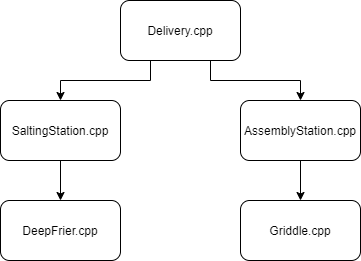
\includegraphics[width=0.5\linewidth]{locks_use.png}
	\caption{Desenho demonstrando como cada módulo usa os \textit{locks} de outros módulos}
	\label{fig:locksUse}
\end{figure}

\begin{lstlisting}[caption=Entrega de pedido no módulo de \textit{Delivery}.\label{lst:orderDelivery}]
bool Delivery::deliverOrder()
{
	bool canDo = false;
	order_t front;
	
	pthread_mutex_lock(&mutex);
	pthread_mutex_lock(&SaltingStation::mutex);
	pthread_mutex_lock(&AssemblyStation::mutex);
	if (ordersQueue.size() > 0)
	{
		
		front = ordersQueue.front();
		
		if (workers < maxWorkers 
			&& SaltingStation::fries >= front.fries 
			&& AssemblyStation::burgers >= front.burgers)
		{
			ordersQueue.pop();
			++workers;
			AssemblyStation::burgers -= front.burgers;
			SaltingStation::fries -= front.fries;
			totalBurgers -= front.burgers;
			totalFries -= front.fries;
			statusDisplayer
				->updateDeliveryWorkers(workers);
			statusDisplayer
				->updateAssemblyStationBurgers(AssemblyStation::burgers);
			statusDisplayer
				->updateSaltingFries(SaltingStation::fries);
			statusDisplayer
				->updateDeliveryOrdered(totalFries, totalBurgers);
			statusDisplayer
				->updateDeliveryFirstOrder(ordersQueue);
			canDo = true;
		}
	}
	pthread_mutex_unlock(&mutex);
	pthread_mutex_unlock(&SaltingStation::mutex);
	pthread_mutex_unlock(&AssemblyStation::mutex);
	
	if (!canDo)
		return false;
	
	sleep(assemblingTime);
	
	// Allows one customer to order more.
	pthread_cond_signal(&waitForOrderDelivered);
	
	pthread_mutex_lock(&mutex);
	if (--workers == maxWorkers - 1)
		Worker::broadcastAvailableTasks();
	statusDisplayer->updateDeliveryWorkers(workers);
	pthread_mutex_unlock(&mutex);
	
	return true;
}	
\end{lstlisting}

\subsection{Evitando esperas ocupadas}
\label{sec:avoidBusyWaits}

Para evitar esperas ocupadas foram usadas variáveis de condição em todas as \textit{threads}. Existem apenas 3 tipos de \textit{threads} nesse programa: a fritadeira, o funcionário e o freguês. O código referente a \textit{thread} da fritadeira se encontra no algoritmo \ref{lst:deepFriersThread} na seção \ref{sec:specialCaseDeepFriers} junto da explicação de como dorme e acorda.

O funcionário fica em busca de tarefas até que não exista absolutamente nenhuma no momento para executar. Na linha 20 do algoritmo \ref{lst:workerThread} ele descobre o que precisa ser feito primeiro e nas linhas 21 a 36 ele tenta em ordem cada uma das prioridades. Caso não seja possível entregar pedidos, executar um passo na linha de produção de batatas fritas ou executar um passo na linha de hambúrgueres, a \textit{thread} do usuário dorme como descrito na linha 38 e 46. O mecanismo para acordar é bem simples, criou-se uma função \texttt{Worker::broadcastAvailableTasks()} que faz um \textit{broadcast} a todos os funcionários dormindo de que há a possibilidade de realizar uma tarefa. Essencialmente sempre que uma tarefa acaba de uma forma que abra espaço para trabalhadores realizarem alguma tarefa que antes não era possível, essa função é chamada e acorda todos os funcionários. A partir daí é uma corrida para fazer tarefas. Dessa forma é evitado que algum funcionário fique incansavelmente tentando fazer cada uma das tarefas, tomando tempo de processamento de outras \textit{threads} úteis.

\begin{lstlisting}[caption=O código executado pela \textit{thread} de funcionário.\label{lst:workerThread}]
void *Worker::Worker(void *args)
{
	std::vector<Delivery::priority_type_t> priorities;
	bool doneSomething;
	
	std::ostringstream out;
	int id = *(int *)args;
	delete (int *)args;
	
	out << "Worker of id " << id << " instantiated" << std::endl;
	if (loggingEnabled)
		logFile << out.str();
	out.str("");
	
	while (runThreads)
	{
		doneSomething = false;
		while (!doneSomething)
		{
			priorities = Delivery::getPriority();
			for (auto priority : priorities)
			{
				switch (priority)
				{
					// Tenta realizar tarefas seguindo ordem de prioridade
					// [...]
				}
				
				if (doneSomething)
				{
					if (loggingEnabled)
						logFile << out.str();
					out.str("");
					break;
				}
			}
			pthread_mutex_lock(&mutex);
			if (!doneSomething)
			{
				out << "Worker[" << id 
					<< "]: Sem tarefas para fazer, vou esperar por uma." 
					<< std::endl;
				if (loggingEnabled)
					logFile << out.str();
				out.str("");
				pthread_cond_wait(&waitForTask, &mutex);
			}
			pthread_mutex_unlock(&mutex);
		}
	}
	return nullptr;
}
\end{lstlisting}

Para os fregueses fica um algoritmo bem mais simples. Pode-se ver no algoritmo \ref{lst:customerThread} que consiste de um produtor que dorme: nas linhas de 16 a 24 o freguês pensa num pedido; na linha 26 ele faz o pedido inserindo numa fila e; na linha 37 ele espera pela entrega do seu pedido. Quando ocorre a entrega de um pedido, sempre acorda-se um freguês. Dessa forma na fila têm-se sempre a quantidade de fregueses em pedidos.

\begin{lstlisting}[caption=Código executado pela \textit{thread} de freguês.\label{lst:customerThread}]
void *Delivery::Customer(void *args)
{
	order_t order;
	std::ostringstream out;
	int id = *(int *)args;
	delete (int *)args;
	
	out << "Customer of id " << id << " instantiated" << std::endl;
	if (loggingEnabled)
		logFile << out.str();
	out.str("");
	
	while (runThreads)
	{
		/* Think of an order */
		order.burgers = 0;
		order.fries = 0;
		while (order.burgers <= 0 && order.fries <= 0)
		{
			order.burgers = random() % 6;
			order.fries = std::max(
				order.burgers + ((int)random() % 5) - 2, 0
			);
		}
		
		placeOrder(order);
		out << "Customer[" << id << "]: Pedi " << order.fries 
			<< " fritas e " << order.burgers << " hamburgueres." 
			<< std::endl;
		if (loggingEnabled)
			logFile << out.str();
		out.str("");
		
		// The customer waits for a delivery to be made 
		// before ordering more.
		pthread_mutex_lock(&orderMakingMutex);
		pthread_cond_wait(&waitForOrderDelivered, &orderMakingMutex);
		pthread_mutex_unlock(&orderMakingMutex);
	}
	
	return nullptr;
}
\end{lstlisting}

Por fim o último mecanismo adotado foi limitar a quantidade de produtos gerados pelas primeiras etapas de produção, a fritadeira e a grelha. As tarefas realmente importantes de salgar as batatas e de montar hambúrgueres criam um gargalo por conta de sua produção mais lenta. Quando se combina isso com um excesso de funcionários, haverá sempre alguém fritando hambúrgueres e fritando batatas, podendo acumular uma quantidade enorme de carnes e batatas. Isso no fim das contas cria uma espécie de espera ocupada em que os funcionários ficam fazendo tarefas sem valor para o momento. Sendo assim foram adicionados mecanismos que limitam a quantidade de fritas sem sal e de carnes de hambúrguer como vistos nas linha 7 e 8 do algoritmo \ref{lst:deepFriersSetup}.

\subsection{Sobre \textit{starvation}}
\label{sec:aboutStarvation}

Este programa está sujeito a \textit{starvations}, sendo alguns casos parte da simulação e outros não relevantes. No caso podem ocorrer quando existem funcionários demais, porém depende muito da sorte, já que teria de ter um grupo de funcionários que ficam se alternando nas tarefas, enquanto os resto não consegue adquirir os \textit{locks} para realizar uma tarefa antes desse pertencentes ao grupo. Esse comportamento é esperado e pode ajudar a mostrar ineficiências na cozinha quando muitos trabalhadores ficam a espera por tarefas. O outro caso é quando se leva em consideração os fregueses, sendo possível que sempre a mesma \textit{thread} seja acordada para fazer outro pedido e a outra fique dormindo. Esse comportamento não é problemático, pois eles estão lá apenas para criar uma espécie de fila infinita de pedidos e fregueses.

Já para as \textit{threads} de fritadeiras, a necessidade de fritas sem sal para a estação de salgagem evitam que elas não possam trabalhar por conta dos trabalhadores. Entre as fritadeiras existe sim a possibilidade de \textit{starvation}, porém não importa muito, pois as outras continuam gerando fritas e pode servir como um indicativo de que há muitas fritadeiras.

\subsection{Exibindo o estado da simulação}
\label{sec:showProgramState}

Por fim o último elemento a explicar é como mostrar o estado do sistema de uma forma geral e menos poluída. Para resolver esse problema foi criada uma classe \texttt{StatusDisplayer} cuja função é fazer isso. Para não ter que reorganizar o programa para gerenciar o estado em um único módulo, optou-se por fazer com que cada mudança nas variáveis interessantes chamasse essa classe atualizando o valor. Sempre que atualiza é escrito na tela o novo estado. Para garantir que sejam registradas \textbf{todas} as mudanças de estado, foi criado um \textit{lock} na própria classe que protege todas as mudanças, forçando que sempre haverá um print correto para cada mudança.

\section{Conclusão}

Este trabalho foi mais grande que o esperado, porém foi possível botar muito bem em prática os mecanismos aprendidos na matéria de programação concorrente. Após criar o programa foi notado que poderia ter sido mais fácil implementar certas partes com semáforos e também praticar melhor o reuso com herança, métodos e funções. Apesar desses pontos de melhoria, o código desenvolvido simula corretamente uma cozinha de \textit{fast-food} seguindo as especificações propostas na seção \ref{sec:definingTheProblem}. Além disso esse programa fornece um algoritmo que aproveita bem a concorrência das \textit{threads}, sem causar \textit{deadlocks} e evitando \textit{starvations} ao máximo.

\nocite{cppreference.com}
\nocite{blaise_barney}
\printbibliography

\end{document}
